\section{Red hogare\~na}
Esta red en principio es muy controlada y solo sabemos que cuenta con un n'umero peque\~no de nodos. La red usa
en su mayoria wi-fi por lo cual es de esperar que el nodo que usamos para monitorear la red reciba amplia cantidad de
paquetes who-has y is-at dado que no hay switches segmentando la red que filtren respuestas is-at de terceros.

El primer experimento, el cual ve la red como una fuente con 2 simbolos unicamente, arroja luego de monitorear la red durante
30 minutos que en ella  la mayor parte del trafico es unicast y solo el 17\% es broadcast.

\begin{tabular}{ r|c|c| }
\multicolumn{1}{r}{}
 &  \multicolumn{1}{c}{frecuencia}
 & \multicolumn{1}{c}{informaci'on} \\
\cline{2-3}
broadcast & 0.17 & 2.56 \\
\cline{2-3}
unicast & 0.83 & 0.27 \\
\cline{2-3}
\end{tabular}
 
Estos valores nos dan una entropia de 0.66 bits (siendo el m'aximo 1 dado que hay 2 simbolos en principio equiprobables) lo
 cual concuerda con las expectativas dado que en una red local hogare\~na se espera ver mas que nada trafico unicast entre
 los nodos y el gateway hacia internet.\\
 
En el segundo experimento, el cual modela la red basado en la direcci'on a resolver en mensajes ARP, usamos la misma captura
utilizada en el experimento anterior. El programa que usamos para analizar los resultados destaco 3 nodos de la red cuando
esperabamos solo 1. El siguiente grafico muestra la informaci'on de cada simbolo y la entropia de la fuente, como se puede
ver hay 3 nodos destacados bajo nuestra definici'on.\\
 
\begin{figure}[!h]
\centering
\caption{Informaci'on red hogare\~na}
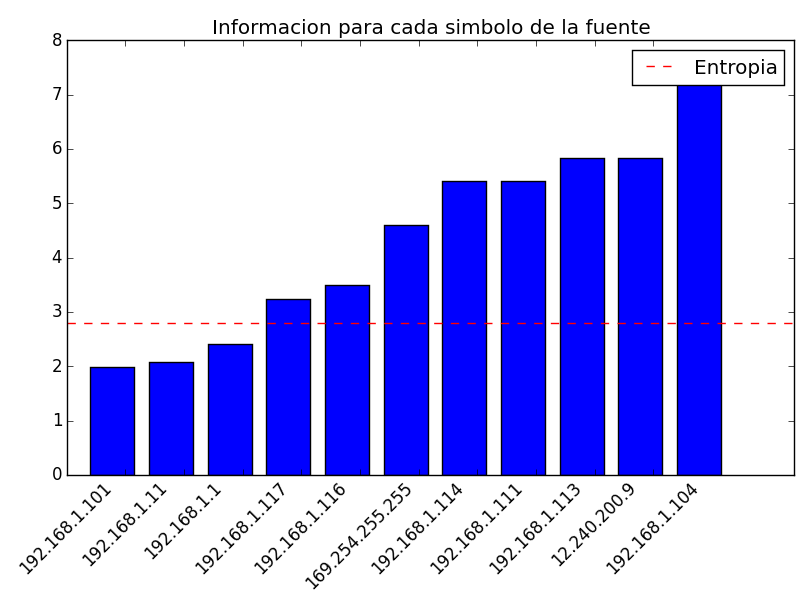
\includegraphics[width=0.55\textwidth]{red1_info}
 \label{fig:red1info}
\end{figure}

Una investigaci'on m'as meticulosa concluyo que \texttt{192.168.1.1} es el gateway por defecto de la red mientras que los otros 2 nodos
destacados, \texttt{192.168.1.11} y \texttt{192.168.1.101} ni siquiera existen en la red, las direcciones no fueron asignadas y ning'un
nodo las esta usando mas un nodo de la red esta constantemente intentando resolver su direcci'on de enlace. Solo podemos
suponer que este host tiene software mal configurado o defectuoso.\\

Las interacciones de los nodos se puede ver en m'as detalle con el siguiente grafico donde se puede ver a los nodos destacados
y las relaciones con los otros nodos. Notar que en el grafico, asi como en el experimento tambi'en aparece un nodo con direcci'on 
\texttt{196.254.255.255} la cual es la direcci'on que el sistema operativo windows asignado a un nodo cuando este no puede
contactar a ning'un servidor DHCP para que le asigne una direcci'on libre. Usualmente los nodos operan con esta direcci'on durante
segundos o minutos hasta que se puedan proveer de una direcci'on valida.\\

\begin{figure}[!h]
\centering
\caption{Visualizaci'on red hogare\~na}
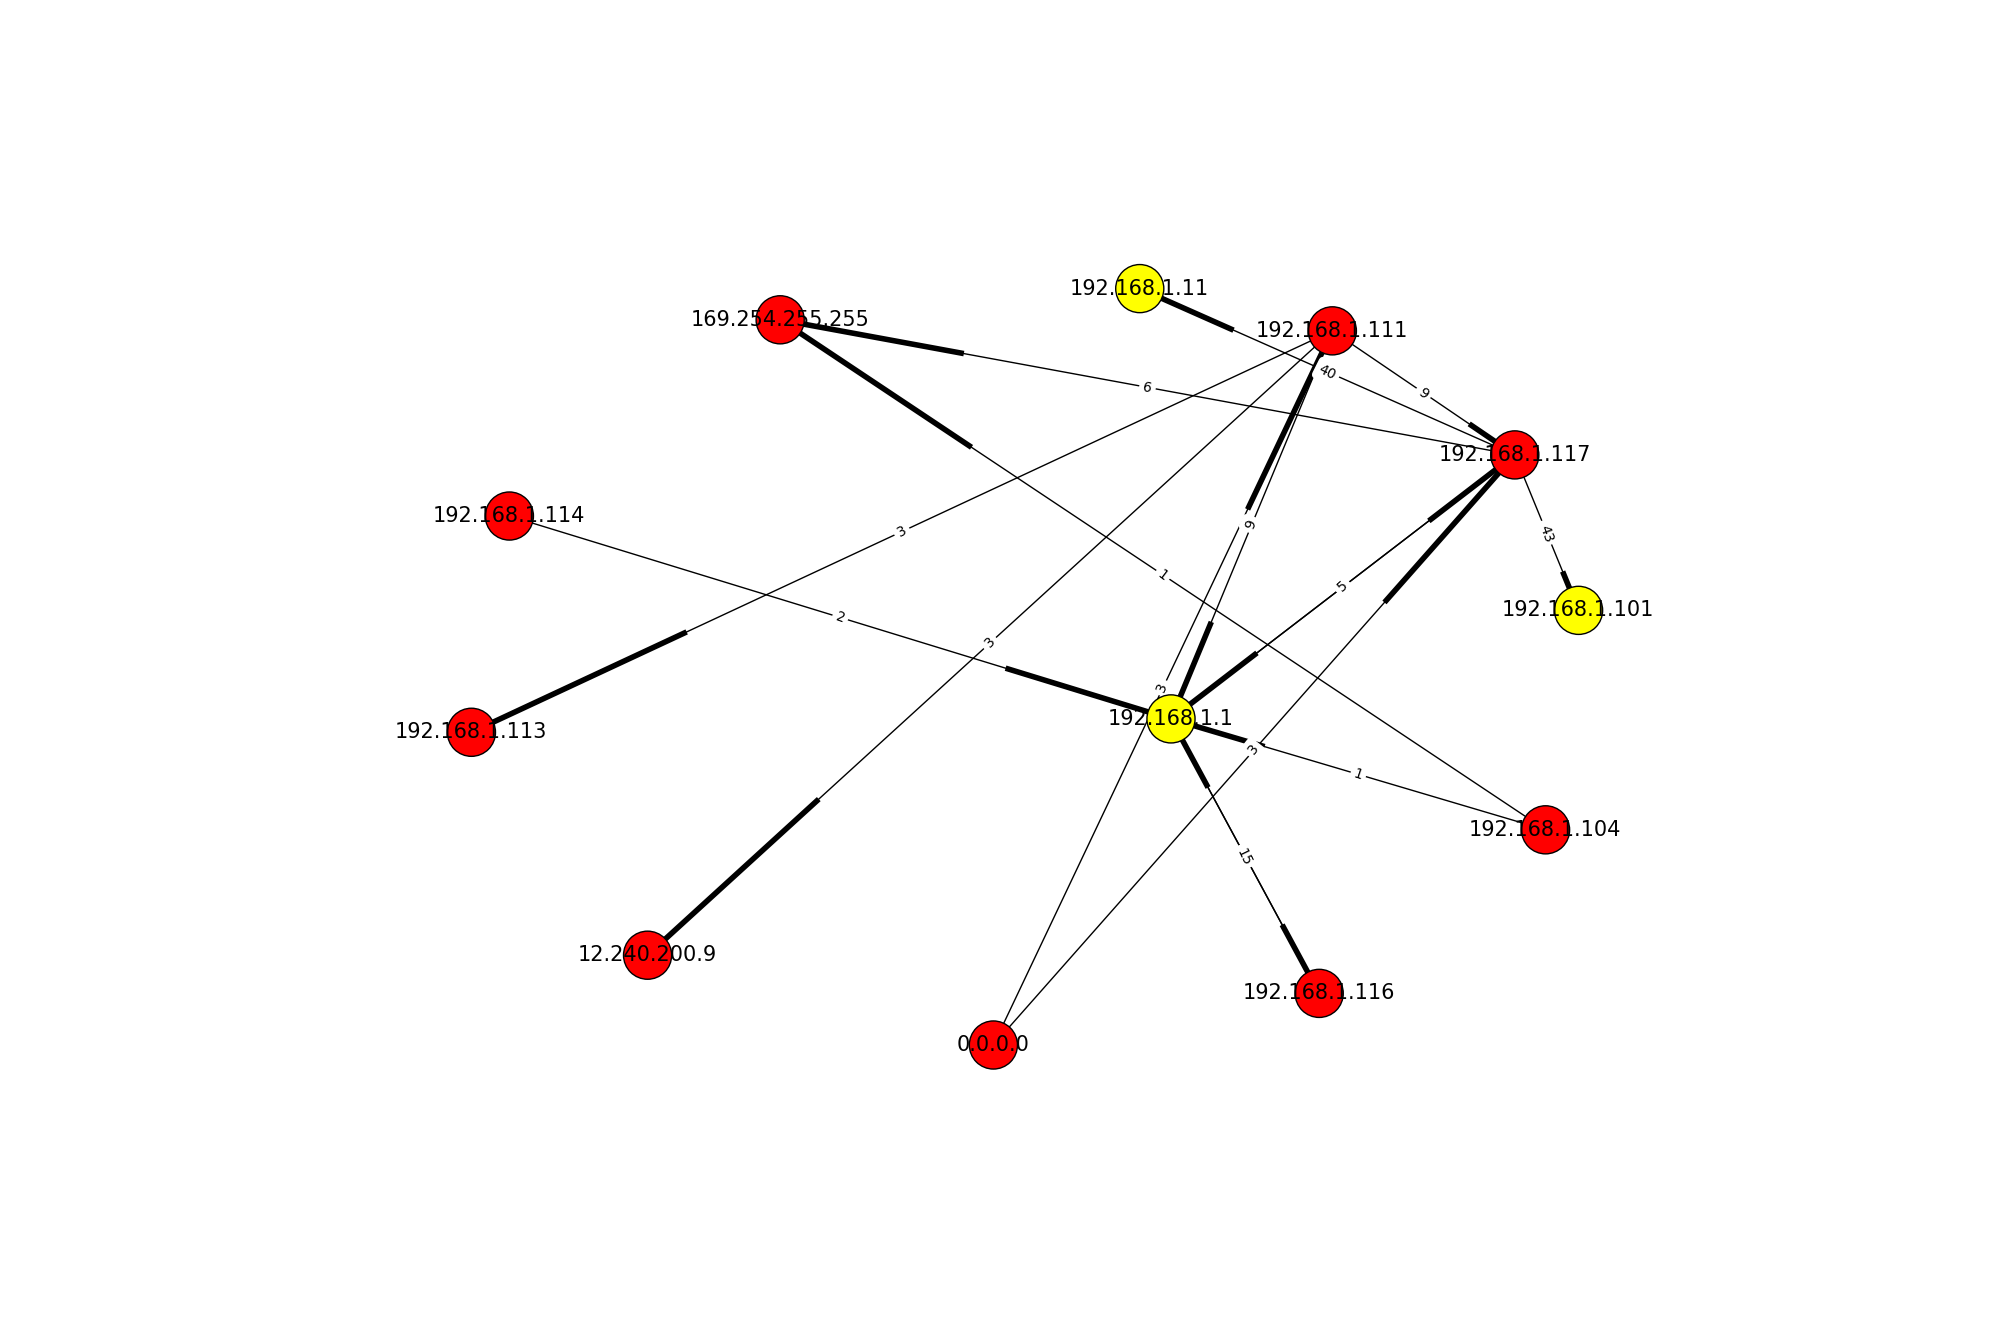
\includegraphics[width=0.9\textwidth]{red1_red}
 \label{fig:red1net}
\end{figure}

El gr'afico confirma que los nodos no existentes que se destacaron son solo accedidos por un nodo.
